\documentclass[12pt,oneside,a4paper,portrait]{article}
\usepackage[a4paper,portrait,margin=1in]{geometry}
\usepackage{tikz}
\usepackage{xcolor}

% Define colors from the original document
\definecolor{cwAlert}{RGB}{235,55,75}
\definecolor{cwDecoy}{RGB}{75,155,235}
\definecolor{cwFlow}{RGB}{155,235,75}
\definecolor{cwBorder}{RGB}{100,100,100}
\definecolor{cwValid}{RGB}{255,215,0}

\begin{document}

\section*{TikZ Test - Fixed Diagrams}

\subsection*{Agent Capabilities (Fixed)}

\begin{figure}[h]
\centering
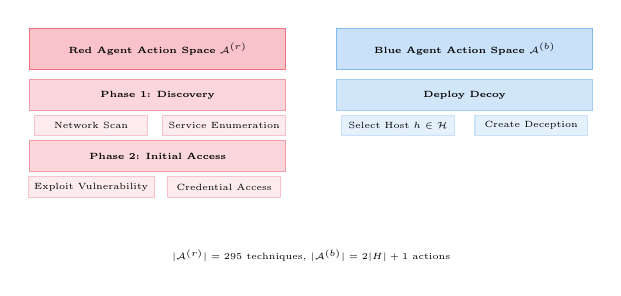
\begin{tikzpicture}[scale=0.65,font=\tiny,node distance=0.6cm,transform shape]
    % Red Agent Kill Chain (Left Side) - using nodes instead of fill
    \node[draw=cwAlert!70,fill=cwAlert!30,rectangle,minimum width=5cm,minimum height=0.8cm,align=center] at (2.5,5.5) {\textbf{Red Agent Action Space} $\mathcal{A}^{(r)}$};
    
    % Phase 1: Discovery
    \node[draw=cwAlert!50,fill=cwAlert!20,rectangle,minimum width=5cm,minimum height=0.6cm,align=center] at (2.5,4.6) {\textbf{Phase 1: Discovery}};
    \node[draw=cwAlert!30,fill=cwAlert!10,rectangle,minimum width=2.2cm,minimum height=0.4cm] at (1.2,4.0) {Network Scan};
    \node[draw=cwAlert!30,fill=cwAlert!10,rectangle,minimum width=2.2cm,minimum height=0.4cm] at (3.8,4.0) {Service Enumeration};
    
    % Phase 2: Initial Access  
    \node[draw=cwAlert!50,fill=cwAlert!20,rectangle,minimum width=5cm,minimum height=0.6cm,align=center] at (2.5,3.4) {\textbf{Phase 2: Initial Access}};
    \node[draw=cwAlert!30,fill=cwAlert!10,rectangle,minimum width=2.2cm,minimum height=0.4cm] at (1.2,2.8) {Exploit Vulnerability};
    \node[draw=cwAlert!30,fill=cwAlert!10,rectangle,minimum width=2.2cm,minimum height=0.4cm] at (3.8,2.8) {Credential Access};
    
    % Blue Agent Actions (Right Side)
    \node[draw=cwDecoy!70,fill=cwDecoy!30,rectangle,minimum width=5cm,minimum height=0.8cm,align=center] at (8.5,5.5) {\textbf{Blue Agent Action Space} $\mathcal{A}^{(b)}$};
    
    % Deploy Action
    \node[draw=cwDecoy!50,fill=cwDecoy!25,rectangle,minimum width=5cm,minimum height=0.6cm,align=center] at (8.5,4.6) {\textbf{Deploy Decoy}};
    \node[draw=cwDecoy!30,fill=cwDecoy!15,rectangle,minimum width=2.2cm,minimum height=0.4cm] at (7.2,4.0) {Select Host $h \in \mathcal{H}$};
    \node[draw=cwDecoy!30,fill=cwDecoy!15,rectangle,minimum width=2.2cm,minimum height=0.4cm] at (9.8,4.0) {Create Deception};
    
    % Mathematical notation
    \node[below=0.3cm] at (5.5,2) {$|\mathcal{A}^{(r)}| = 295$ techniques, $|\mathcal{A}^{(b)}| = 2|H| + 1$ actions};
\end{tikzpicture}
\caption{Agent Capabilities Test - Text should be visible on colored backgrounds}
\end{figure}

\end{document}
